% 固定来源PDF印刷页52第24题圆柱、轴截面和垂足的矢量示意重绘。
% 使用斜投影表达拓扑关系；圆柱比例不代表题设精确度量。
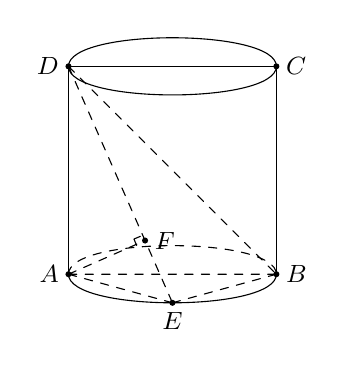
\begin{tikzpicture}[x=.88cm,y=.88cm,font=\small,line cap=round,line join=round]
  \coordinate (A) at (-1.5,0);
  \coordinate (B) at (1.5,0);
  \coordinate (C) at (1.5,3);
  \coordinate (D) at (-1.5,3);
  \coordinate (E) at (0,-.4125);
  \coordinate (F) at (-.395,.486);

  % Cylinder sides and top circular rim.
  \draw (A)--(D) (B)--(C);
  \draw (D) .. controls (-1.5,3.55) and (1.5,3.55) .. (C);
  \draw (D)--(C);
  \draw (D) .. controls (-1.5,2.45) and (1.5,2.45) .. (C);
  % The rear half of the lower rim is hidden; the near half is visible.
  \draw[dashed] (A) .. controls (-1.5,.55) and (1.5,.55) .. (B);
  \draw (A) .. controls (-1.5,-.55) and (1.5,-.55) .. (B);

  % Axial-section diagonal, the perpendicular construction and its foot.
  \draw[dashed] (A)--(B) (D)--(B) (D)--(E) (A)--(F) (A)--(E) (B)--(E);
  % Small right-angle marker at F, fitted to the schematic projections of AF and DE.
  \draw (-.5165,.4155)--(-.5554,.5076)--(-.4633,.5465);
  \fill (A) circle (1.1pt) (B) circle (1.1pt) (C) circle (1.1pt)
        (D) circle (1.1pt) (E) circle (1.1pt) (F) circle (1.1pt);
  \node[left] at (A) {$A$};
  \node[right] at (B) {$B$};
  \node[right] at (C) {$C$};
  \node[left] at (D) {$D$};
  \node[below] at (E) {$E$};
  \node[right] at (F) {$F$};
\end{tikzpicture}
